\PassOptionsToPackage{unicode=true}{hyperref} % options for packages loaded elsewhere
\PassOptionsToPackage{hyphens}{url}
%
\documentclass[10pt,xcolor=table,color={dvipsnames,usenames},ignorenonframetext,usepdftitle=false,french]{beamer}
\setbeamertemplate{caption}[numbered]
\setbeamertemplate{caption label separator}{: }
\setbeamercolor{caption name}{fg=normal text.fg}
\beamertemplatenavigationsymbolsempty
\usepackage{caption}
\captionsetup{skip=0pt,belowskip=0pt}
%\setlength\abovecaptionskip{-15pt}
\usepackage{lmodern}
\usepackage{amssymb,amsmath,mathtools,multirow}
\usepackage{float,hhline}
\usepackage{tikz}
\usepackage[tikz]{bclogo}
\usepackage{mathtools}
\usepackage{ifxetex,ifluatex}
\usepackage{fixltx2e} % provides \textsubscript
\ifnum 0\ifxetex 1\fi\ifluatex 1\fi=0 % if pdftex
  \usepackage[T1]{fontenc}
  \usepackage[utf8]{inputenc}
  \usepackage{textcomp} % provides euro and other symbols
\else % if luatex or xelatex
  \usepackage{unicode-math}
  \defaultfontfeatures{Ligatures=TeX,Scale=MatchLowercase}
\fi
\usetheme[coding=utf8,language=french,
,titlepagelogo=img/LOGO-ENSAE.png
]{TorinoTh}
% use upquote if available, for straight quotes in verbatim environments
\IfFileExists{upquote.sty}{\usepackage{upquote}}{}
% use microtype if available
\IfFileExists{microtype.sty}{%
\usepackage[]{microtype}
\UseMicrotypeSet[protrusion]{basicmath} % disable protrusion for tt fonts
}{}
\IfFileExists{parskip.sty}{%
\usepackage{parskip}
}{% else
\setlength{\parindent}{0pt}
\setlength{\parskip}{6pt plus 2pt minus 1pt}
}
\usepackage{hyperref}
\hypersetup{
            pdftitle={Itinéraire entre deux stations du métro parisien},
            pdfauthor={Kim Antunez et Alain Quartier-la-Tente},
            pdfborder={0 0 0},
            breaklinks=true}
\urlstyle{same}  % don't use monospace font for urls
\newif\ifbibliography
% Prevent slide breaks in the middle of a paragraph:
\widowpenalties 1 10000
\raggedbottom
\AtBeginPart{
  \let\insertpartnumber\relax
  \let\partname\relax
  \frame{\partpage}
}
\setlength{\emergencystretch}{3em}  % prevent overfull lines
\providecommand{\tightlist}{%
  %\setlength{\itemsep}{0pt}
  \setlength{\parskip}{0pt}
  }
\setcounter{secnumdepth}{0}

% set default figure placement to htbp
\makeatletter
\def\fps@figure{htbp}
\makeatother

\usepackage{wrapfig}
\usepackage{booktabs}
\usepackage{longtable}
\usepackage{array}
\usepackage{multirow}
\usepackage[table]{xcolor}
\usepackage{wrapfig}
\usepackage{float}
\usepackage{colortbl}
\usepackage{pdflscape}
\usepackage{tabu}
\usepackage{threeparttable}
\usepackage{threeparttablex}
\usepackage[normalem]{ulem}
\usepackage{makecell}
\usepackage{animate}
\usepackage{fontawesome5}

\title{Itinéraire entre deux stations du métro parisien}
\ateneo{Projet C++, Ensae}
\author{Kim Antunez et Alain Quartier-la-Tente}
\date{}


\setrellabel{}

\setcandidatelabel{}

\rel{}
\division{07/01/2020 - 15h30 à 15h45}

\departement{Ensae --- 2019-2020}
\makeatletter
\let\@@magyar@captionfix\relax
\makeatother

\DeclareMathOperator{\Cov}{Cov}
\newcommand{\E}[1]{\mathbb{E}\left[ #1 \right]}
\newcommand{\V}[1]{\mathbb{V}\left[ #1 \right]}
\newcommand{\cov}[2]{\Cov\left( #1\,,\,#2 \right)}

\begin{document}
\begin{frame}[plain,noframenumbering]
\titlepage
\end{frame}

\begin{frame}{Sommaire}
\protect\hypertarget{sommaire}{}

\tableofcontents

\end{frame}

\hypertarget{description-des-classes}{%
\section{Description des classes}\label{description-des-classes}}

\begin{frame}{Description des classes}
\protect\hypertarget{description-des-classes-1}{}

\end{frame}

\hypertarget{description-de-lalgorithme}{%
\section{Description de l'algorithme}\label{description-de-lalgorithme}}

\begin{frame}{Description de l'algorithme (1/8)}
\protect\hypertarget{description-de-lalgorithme-18}{}

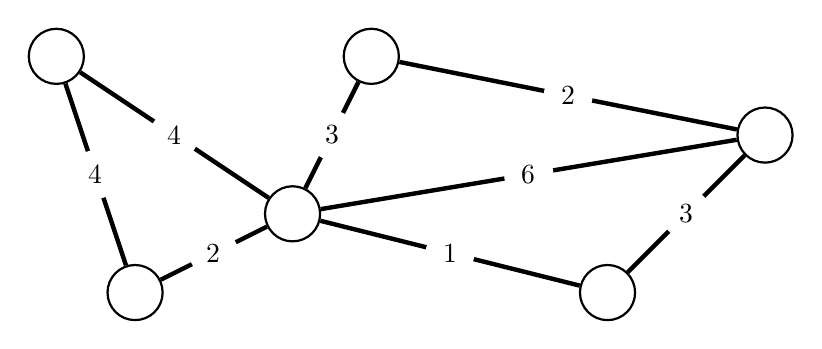
\begin{tikzpicture}
\begin{scope}[every node/.style={circle,thick,draw,minimum size=0.7cm}]
    \node (A) at (0,0) {};
    \node (B) at (1,-3) {};
    \node (C) at (3,-2) {};
    \node (D) at (4,0) {};
    \node (E) at (7,-3) {};
    \node (F) at (9,-1) {} ;
\end{scope}

\begin{scope}[
              every node/.style={fill=white,circle},
              every edge/.style={draw=black,ultra thick}]
    \path  (A) edge node {$4$} (B);
    \path  (B) edge node {$2$} (C);
    \path  (A) edge node {$4$} (C);
    \path  (C) edge node {$3$} (D);
    \path  (C) edge node {$1$} (E);
    \path  (C) edge node {$6$} (F);
    \path  (D) edge node {$2$} (F);
    \path  (E) edge node {$3$} (F);
\end{scope}
\end{tikzpicture}

\end{frame}

\begin{frame}{Description de l'algorithme (2/8)}
\protect\hypertarget{description-de-lalgorithme-28}{}

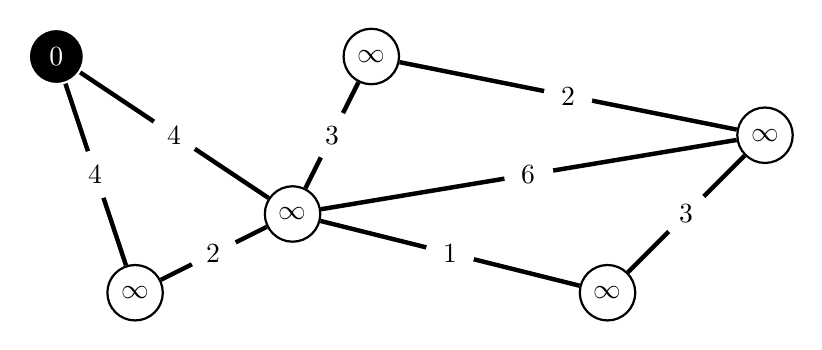
\begin{tikzpicture}
\begin{scope}[every node/.style={circle,thick,draw,minimum size=0.7cm}]
    \node (A)[white, thick,draw,fill=black] at (0,0) {0};
    \node (B) at (1,-3) {$\infty$};
    \node (C) at (3,-2) {$\infty$};
    \node (D) at (4,0) {$\infty$};
    \node (E) at (7,-3) {$\infty$};
    \node (F) at (9,-1) {$\infty$} ;
\end{scope}

\begin{scope}[every node/.style={fill=white,circle},
              every edge/.style={draw=black,ultra thick}]
    \path  (A) edge node {$4$} (B);
    \path  (B) edge node {$2$} (C);
    \path  (A) edge node {$4$} (C);
    \path  (C) edge node {$3$} (D);
    \path  (C) edge node {$1$} (E);
    \path  (C) edge node {$6$} (F);
    \path  (D) edge node {$2$} (F);
    \path  (E) edge node {$3$} (F);
\end{scope}
\end{tikzpicture}

\end{frame}

\begin{frame}{Description de l'algorithme (3/8)}
\protect\hypertarget{description-de-lalgorithme-38}{}

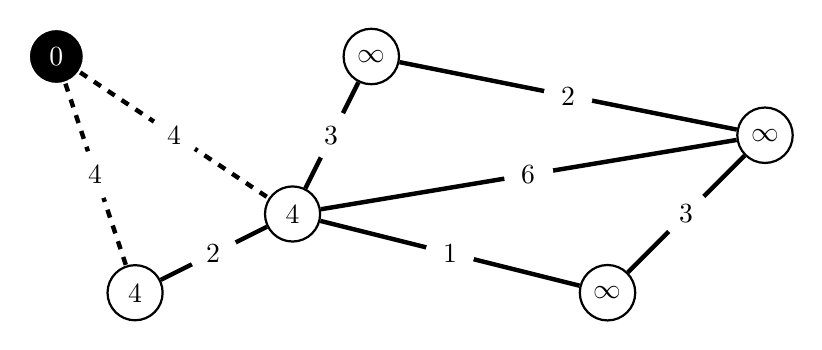
\begin{tikzpicture}
\begin{scope}[every node/.style={circle,thick,draw,minimum size=0.7cm}]
    \node (A)[white, thick,draw,fill=black] at (0,0) {0};
    \node (B) at (1,-3) {4};
    \node (C) at (3,-2) {4};
    \node (D) at (4,0) {$\infty$};
    \node (E) at (7,-3) {$\infty$};
    \node (F) at (9,-1) {$\infty$} ;
\end{scope}

\begin{scope}[
              every node/.style={fill=white,circle},
              every edge/.style={draw=black,ultra thick}]
    \path  (A) edge[dashed] node {$4$} (B);
    \path  (B) edge node {$2$} (C);
    \path  (A) edge[dashed] node {$4$} (C);
    \path  (C) edge node {$3$} (D);
    \path  (C) edge node {$1$} (E);
    \path  (C) edge node {$6$} (F);
    \path  (D) edge node {$2$} (F);
    \path  (E) edge node {$3$} (F);
\end{scope}
\end{tikzpicture}

\end{frame}

\begin{frame}{Description de l'algorithme (4/8)}
\protect\hypertarget{description-de-lalgorithme-48}{}

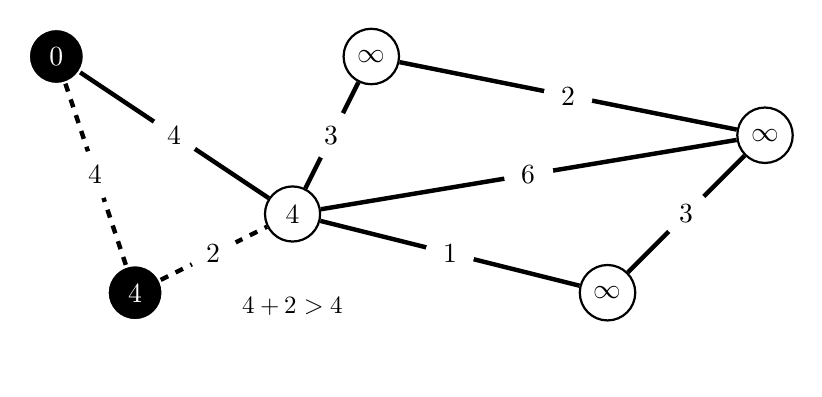
\begin{tikzpicture}
\begin{scope}[every node/.style={circle,thick,draw,minimum size=0.7cm}]
    \node (A)[white, thick,draw,fill=black] at (0,0) {0};
    \node (B)[white, thick,draw,fill=black] at (1,-3) {4};
    \node (C)[label distance=0.1cm, label={below:\small $4+2>4$}] at (3,-2) {4};
    \node (D) at (4,0) {$\infty$};
    \node (E) at (7,-3) {$\infty$};
    \node (F) at (9,-1) {$\infty$} ;
\end{scope}

\begin{scope}[
              every node/.style={fill=white,circle},
              every edge/.style={draw=black,ultra thick}]
    \path  (A) edge[dashed] node {$4$} (B);
    \path  (B) edge[dashed] node {$2$} (C);
    \path  (A) edge node {$4$} (C);
    \path  (C) edge node {$3$} (D);
    \path  (C) edge node {$1$} (E);
    \path  (C) edge node {$6$} (F);
    \path  (D) edge node {$2$} (F);
    \path  (E) edge node {$3$} (F);
\end{scope}
\end{tikzpicture}

\end{frame}

\begin{frame}{Description de l'algorithme (5/8)}
\protect\hypertarget{description-de-lalgorithme-58}{}

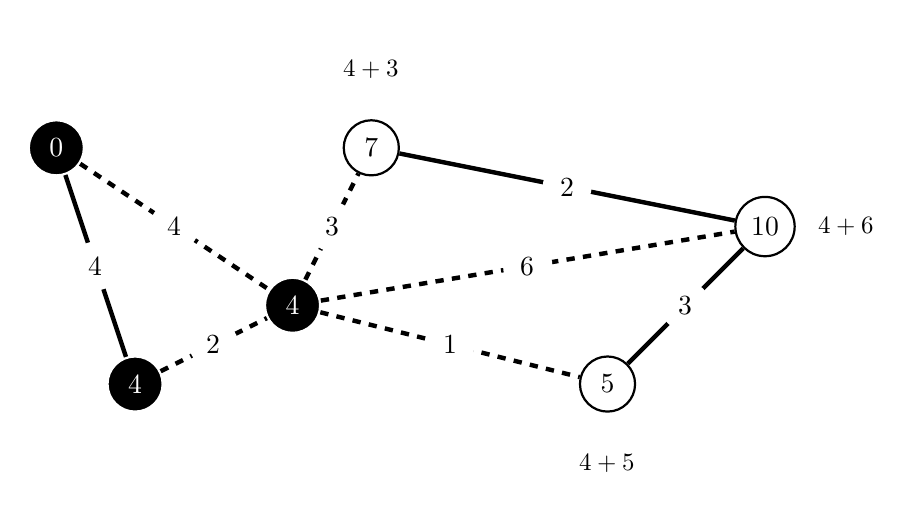
\begin{tikzpicture}
\begin{scope}[every node/.style={circle,thick,draw,minimum size=0.7cm}]
    \node (A)[white, thick,draw,fill=black] at (0,0) {0};
    \node (B)[white, thick,draw,fill=black] at (1,-3) {4};
    \node (C)[white, thick,draw,fill=black] at (3,-2) {4};
    \node (D)[label={[label distance=0.1cm]\small $4+3$}] at (4,0) {7};
    \node (E)[label={[label distance=0.1cm]below:\small $4+5$}] at (7,-3) {5};
    \node (F)[label={[label distance=0.1cm]right:\small $4+6$}] at (9,-1) {10} ;
\end{scope}

\begin{scope}[
              every node/.style={fill=white,circle},
              every edge/.style={draw=black,ultra thick}]
    \path  (A) edge node {$4$} (B);
    \path  (B) edge[dashed] node {$2$} (C);
    \path  (A) edge[dashed] node {$4$} (C);
    \path  (C) edge[dashed] node {$3$} (D);
    \path  (C) edge[dashed] node {$1$} (E);
    \path  (C) edge[dashed] node {$6$} (F);
    \path  (D) edge node {$2$} (F);
    \path  (E) edge node {$3$} (F);
\end{scope}
\end{tikzpicture}

\end{frame}

\begin{frame}{Description de l'algorithme (6/8)}
\protect\hypertarget{description-de-lalgorithme-68}{}

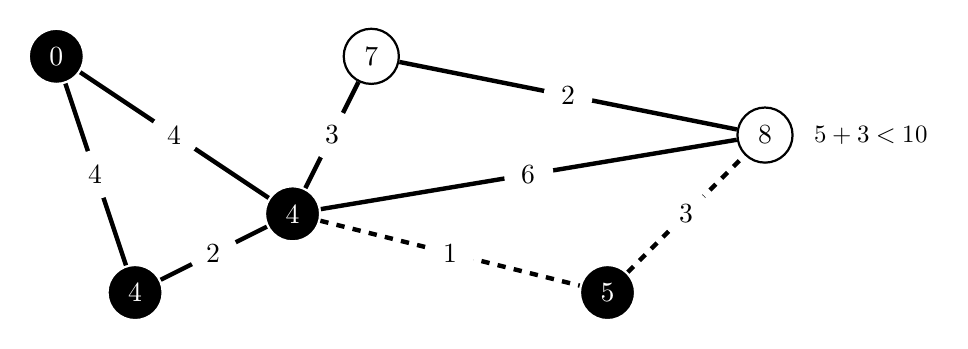
\begin{tikzpicture}
\begin{scope}[every node/.style={circle,thick,draw,minimum size=0.7cm}]
    \node (A)[white, thick,draw,fill=black] at (0,0) {0};
    \node (B)[white, thick,draw,fill=black] at (1,-3) {4};
    \node (C)[white, thick,draw,fill=black] at (3,-2) {4};
    \node (D) at (4,0) {7};
    \node (E)[white, thick,draw,fill=black] at (7,-3) {5};
    \node (F)[label={[label distance=0.1cm]right:\small $5+3<10$}] at (9,-1) {8} ;
\end{scope}

\begin{scope}[
              every node/.style={fill=white,circle},
              every edge/.style={draw=black,ultra thick}]
    \path  (A) edge node {$4$} (B);
    \path  (B) edge node {$2$} (C);
    \path  (A) edge node {$4$} (C);
    \path  (C) edge node {$3$} (D);
    \path  (C) edge[dashed] node {$1$} (E);
    \path  (C) edge node {$6$} (F);
    \path  (D) edge node {$2$} (F);
    \path  (E) edge[dashed] node {$3$} (F);
\end{scope}
\end{tikzpicture}

\end{frame}

\begin{frame}{Description de l'algorithme (7/8)}
\protect\hypertarget{description-de-lalgorithme-78}{}

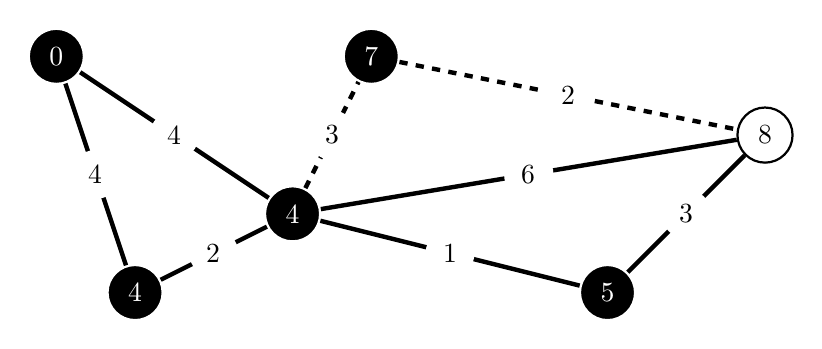
\begin{tikzpicture}
\begin{scope}[every node/.style={circle,thick,draw,minimum size=0.7cm}]
    \node (A)[white, thick,draw,fill=black] at (0,0) {0};
    \node (B)[white, thick,draw,fill=black] at (1,-3) {4};
    \node (C)[white, thick,draw,fill=black] at (3,-2) {4};
    \node (D)[white, thick,draw,fill=black] at (4,0) {7};
    \node (E)[white, thick,draw,fill=black] at (7,-3) {5};
    \node (F) at (9,-1) {8} ;
\end{scope}

\begin{scope}[
              every node/.style={fill=white,circle},
              every edge/.style={draw=black,ultra thick}]
    \path  (A) edge node {$4$} (B);
    \path  (B) edge node {$2$} (C);
    \path  (A) edge node {$4$} (C);
    \path  (C) edge[dashed] node {$3$} (D);
    \path  (C) edge node {$1$} (E);
    \path  (C) edge node {$6$} (F);
    \path  (D) edge[dashed] node {$2$} (F);
    \path  (E) edge node {$3$} (F);
\end{scope}
\end{tikzpicture}

\end{frame}

\begin{frame}{Description de l'algorithme (8/8)}
\protect\hypertarget{description-de-lalgorithme-88}{}

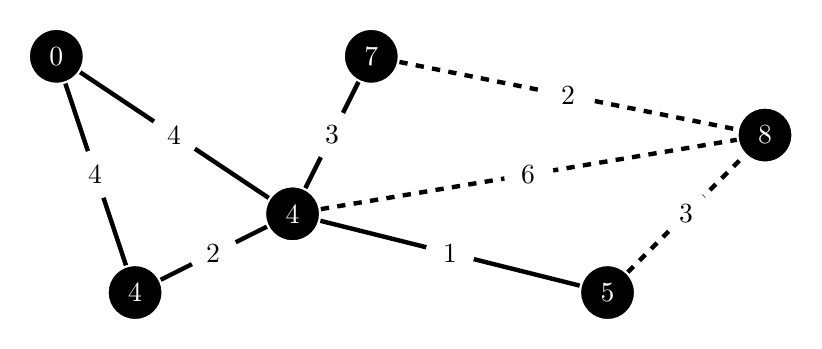
\begin{tikzpicture}
\begin{scope}[every node/.style={circle,thick,draw,minimum size=0.7cm}]
    \node (A)[white, thick,draw,fill=black] at (0,0) {0};
    \node (B)[white, thick,draw,fill=black] at (1,-3) {4};
    \node (C)[white, thick,draw,fill=black] at (3,-2) {4};
    \node (D)[white, thick,draw,fill=black] at (4,0) {7};
    \node (E)[white, thick,draw,fill=black] at (7,-3) {5};
    \node (F)[white, thick,draw,fill=black] at (9,-1) {8} ;
\end{scope}

\begin{scope}[
              every node/.style={fill=white,circle},
              every edge/.style={draw=black,ultra thick}]
    \path  (A) edge node {$4$} (B);
    \path  (B) edge node {$2$} (C);
    \path  (A) edge node {$4$} (C);
    \path  (C) edge node {$3$} (D);
    \path  (C) edge node {$1$} (E);
    \path  (C) edge[dashed] node {$6$} (F);
    \path  (D) edge[dashed] node {$2$} (F);
    \path  (E) edge[dashed] node {$3$} (F);
\end{scope}
\end{tikzpicture}

\end{frame}

\hypertarget{pistes-damuxe9lioration}{%
\section{Pistes d'amélioration}\label{pistes-damuxe9lioration}}

\begin{frame}[fragile]{Pistes d'amélioration}
\protect\hypertarget{pistes-damuxe9lioration-1}{}

\begin{enumerate}
\item
  Améliorer le chargement des données
\item
  Prendre en compte l'horaire (ajout des temps de passage dans
  \texttt{Edge})
\item
  Ajouter d'autres types d'itinéraires
\end{enumerate}

\end{frame}

\end{document}
